\section{Approach}	\label{sec:related_works}

The algorithmic structure of MABDI can be seen in Fig. \ref{fig:system}. The
diagram is very similar to Fig. \ref{fig:pipeline} with the exception of the
Classification component, shown in blue. This Classification component is
MABDI's contribution to the state-of-art in mesh based mapping algorithms, and
is what gives MABDI the ability to make decisions about the incoming data.

The Classification component consists of two elements:
\begin{enumerate}
    \item \textit{Generate Expected Depth Image $E$} - Here we take the global
    mesh $M$, render it using computer graphics, and use the depth buffer of the
    render window to create a depth image $E$ of what we expect to see from our
    sensor. This method requires the current pose $P$ of the actual sensor
    (simulated for our experiments).
    \item \textit{Classify Depth Image $D$} - Here we classify the actual depth
    image $D$ (simulated for our experiments) by first taking the absolute
    difference between $E$ and $D$ and thresholding. If the differences are
    small, those points are thrown away and if the differences are large, those
    points are kept as $D_n$. The idea behind this is, if the difference is
    large, the measurements are coming from a part of the environment that has
    not been seen before i.e., novel. The implication of this assumption is that
    this version of MABDI can not handle object removal. It is worth noting
    that MABDI can be extended to handle object removal by using the sign of the
    difference between $E$ and $D$ instead of the absolute value.
\end{enumerate}

\begin{figure}[h]%[thpb]
\centering
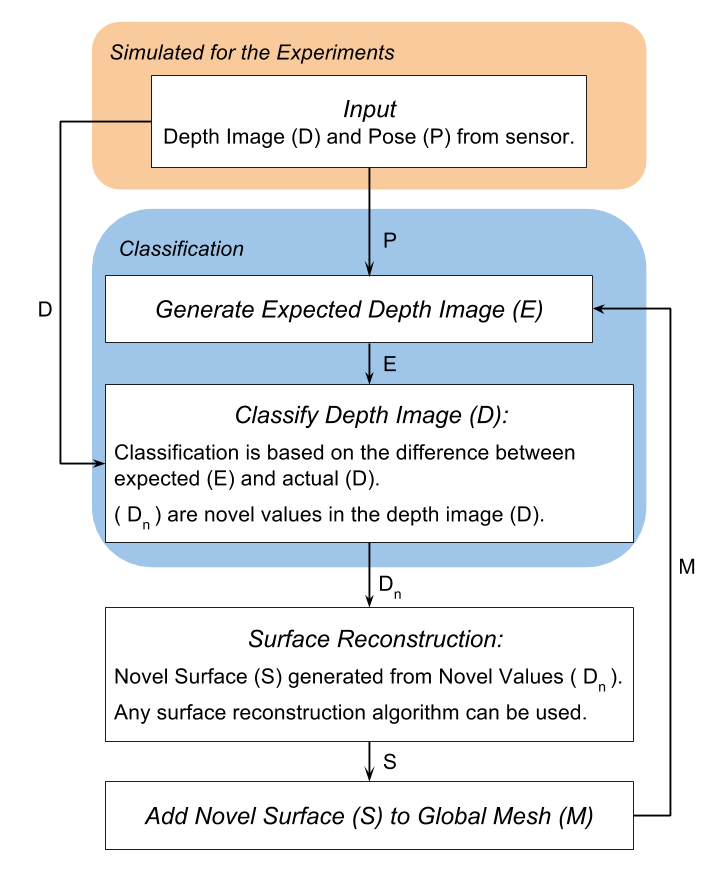
\includegraphics[width=.5\textwidth]{figures/diagram_system.png}
\caption{MABDI system diagram}
\label{fig:system}
\end{figure}

From a software perspective, the major difficulty of implementing the MABDI
algorithm was found to be creating both the simulated depth image $D$ and the
expected depth image $E$. In addition, managing the complexity of the data
pipeline needed to run the algorithm and the simulation of the sensor proved to
be quite overwhelming. Thankfully, Kitware, who is a leading
edge developer of open-source software, created the Visualization Toolkit (VTK)
\cite{schroeder2004visualization, sitevtk}. At the time of this writing the VTK
Github repository has over 60,000 commits and is contributed to by supporters
such as Sandia National Labs \cite{sitevtkoverview}.

MABDI is implemented with Python and uses VTK. The code is freely
available on my Github account \cite{sitemabdi}. At the time of this writing, it
consists of over 1,400 lines. The code that implements the MABDI algorithm
itself is around 750 lines.

VTK is aptly designed for the implementation of MABDI for many reasons. Perhaps
the most important is the concept of a vtkAlgorithm (often called a Filter).
This allows a programmer to create a custom and modular processing pipeline by
defining classes that inherit vtkAlgorithm and then defining the connections
between these classes. For example, you could have a pipeline that reads an
image from a source (component 1), performs edge detection (component 2), and then
renders the image (component 3). Using this concept, the individual elements of
MABDI can be succinctly defined in individual classes. With that in mind, we can
see in Fig. \ref{fig:software} the layout used in my implementation of MABDI:

\begin{itemize}
    \item  \textit{Source} - Classes with the prefix Source define the environment that is used for the simulation and provide a mesh in the form of a vtkPolyData.
    \item \textit{FilterDepthImage} - Render the incoming vtkPolyData in a window and output the depth buffer from the window as a vtkImageData. The output additionally has pose information of the sensor.
    \item \textit{FilterClassifier} - Implements the true innovation of MABDI, takes the difference between the two incoming depth images (vtkImageData) and outputs a new depth image where the data that is not novel is marked to be thrown away.
    \item \textit{FilterDepthImageToSurface} - Performs surface reconstruction on the novel points. In this simple implementation the topology of the mesh is defined in the image coordinates and can be thought of as a checkerboard pattern with two triangles in every square. The data is then projected to real-world coordinates. The topology and the real-world coordinates are combined to define a surface and output as a vtkPolyData.
    \item \textit{FilterWorldMesh} - Here we simply append the incoming novel surface to a growing global mesh that is also output as a vtkPolyData.
\end{itemize}

\begin{figure}[h]%[thpb]
\centering
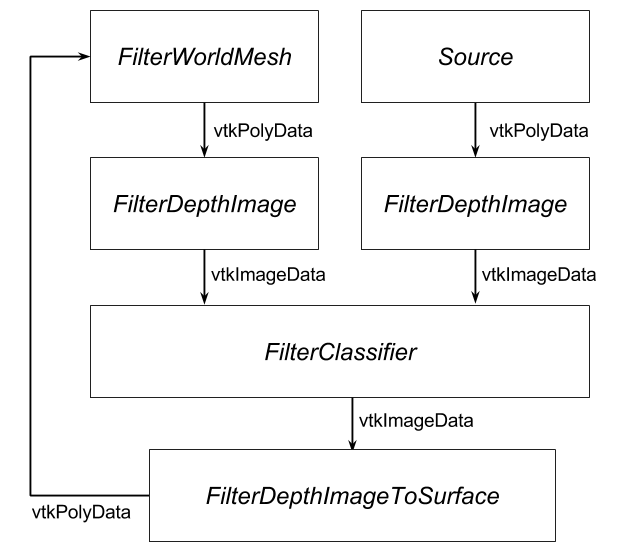
\includegraphics[width=.5\textwidth]{figures/diagram_software.png}
\caption{MABDI software diagram}
\label{fig:software}
\end{figure}
